The random subset problem randomly partitions network space into consensus sets, imposing a subset-sum constraint on consensus set sizes. In the context of symmetric load where all nodes request $|\mathcal{C}|$ consensus load the net consensus load is,
\begin{align}
	L = |\mathcal{C}| \cdot |\mathcal{N}|.
\end{align}
This requires performing $|\mathcal{C}|$ independent re-partitionings within each of which every node will be assigned exactly once. Under this allocation every node both contributes and requests $|\mathcal{C}|$ units of work.

The \emph{consensus assignment problem} generalises the random subset problem to accommodate arbitrary consensus set sizes and asymmetric load, allowing nodes to contribute and request arbitrary consensus workload, a prerequisite for enabling a free consensus market.

Representing consensus assignment via \emph{consensus assignment graphs} (Sec.~\ref{sec:assign_graphs}) reflecting the contributed and requested load by nodes and consensus sets, the algorithm uniformly samples from the space of satisfying assignments (Sec.~\ref{sec:uniform_consensus_samp}), achieved by defining consensus assignment via its algebraic group structure (Sec.~\ref{sec:assign_group}) and uniformly sampling the group action acting on an initial graph assignment (Sec.~\ref{sec:initial_graph_assignment}), where the pseudo-random algorithm is seeded (Sec.~\ref{sec:random_bitstreams}) by a secure random variable established by the network (Sec.~\ref{sec:secure_shared_randomness}) to ensure consistent evaluation in a distributed context. The distributed algorithm for the consensus assignment problem is shown in Alg.~\ref{alg:uniform_consensus_sampling}.

\begin{algorithm}[H]
	\begin{algorithmic}
		\Function{DistConsensusSampling}{$\mathcal{N}$, $U$, $V$, $d$} $\to E$
		\State $\mathcal{X}_\mathcal{N} \gets \textsc{SecureSharedRandomness}(\mathcal{N})$
		\State $E \gets \textsc{CanonicalGraph}(U,V,d)$
		\State $E \gets \textsc{ConsensusShuffle}(\mathcal{X}_\mathcal{N}, E)$
		\State \Return $E$
		\EndFunction
	\end{algorithmic}
	\caption{Distributed algorithm for the consensus assignment problem. A secure shared random variable (Sec.~\ref{sec:secure_shared_randomness}), $\mathcal{X}_\mathcal{N}$, collectively established by the network, $\mathcal{N}$, seeds pseudo-random sampling (Sec.~\ref{sec:uniform_consensus_samp}) over consensus assignments, $E$, satisfying the consensus assignment graph constraints, $(U,V,d)$ (Sec.~\ref{sec:assign_graphs}).} \label{alg:uniform_consensus_sampling}
\end{algorithm}

\subsection{Consensus assignment graphs} \label{sec:assign_graphs}

\begin{figure}[!htb]
	\centering
	\begin{tikzpicture}[genericStyle, every node/.style={circle, draw, minimum size=2em}]
    \def\UVsep{2.8}

    \foreach \i in {1,...,5} {
            \node[draw=none] (a\i) at (0,-\i) {};
        }
    \foreach \i in {1,...,5} {
            \node[draw=none] (b\i) at (\UVsep,-\i) {};
        }

    \node[nodeNetworkStyle, rectangle, rounded corners=5pt, fit=(a1) (a5), inner sep=4pt] (rectU) {};
    \node[nodeConsensusStyle, rectangle, rounded corners=5pt, fit=(b1) (b5), inner sep=4pt] (rectV) {};

    \node[draw=none, above=-0.2em of rectU] (labelU) {$U$};
    \node[draw=none, above=-0.2em of rectV] (labelV) {$V$};
    \node[draw=none] at ($(labelU)!0.5!(labelV)$) {$E$};

    \node[nodeGrayStyle] (a1) at (0,-1) {};
    \node[nodeGrayStyle] (a2) at (0,-2) {$u_i$};
    \node[nodeGrayStyle] (a3) at (0,-3) {};
    \node[draw=none] (a4) at (0,-4) {\LARGE $\vdots$};
    \node[nodeGrayStyle] (a5) at (0,-5) {};

    \node[nodeGrayStyle] (b1) at (\UVsep,-1) {};
    \node[nodeGrayStyle] (b2) at (\UVsep,-2) {};
    \node[nodeGrayStyle] (b3) at (\UVsep,-3) {$v_j$};
    \node[draw=none] (b4) at (\UVsep,-4) {\LARGE $\vdots$};
    \node[nodeGrayStyle] (b5) at (\UVsep,-5) {};

    \foreach \i in {1,...,5} {
            \foreach \j in {1,...,5} {
                    \draw[graphNonEdgeStyle] ($(rectU.east |- a\i) + (0.01,0)$) -- ($(rectV.west |- b\j) + (-0.01,0)$);
                }
        }

    \draw[->, black, line width=0.8, line cap=round] (rectU.east |- a2) -- node[draw=none, draw=none, text=black, above=-1em,midway] {$e=(u_i,v_j)$} (rectV.west |- b3);
\end{tikzpicture}
	%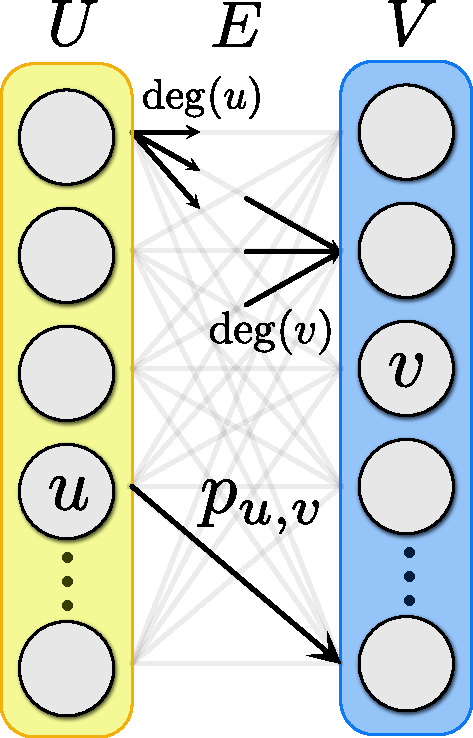
\includegraphics[width=0.4\columnwidth]{figures/bipartite_map.pdf}
	\caption{\textbf{Generalised consensus assignment problem.} Consensus assignment may be represented as a directed bipartite graph, \mbox{$\mathcal{G}=(U,V,E)$}, from a space of network nodes, $U\equiv\mathcal{N}$, to consensus sets, $V\equiv\{\mathcal{C}\}$, where vertex degree represents contributed/consumed consensus load. The set of all satisfying edge-sets $\{E\}$ represents the space of valid assignments. Under sampling, $p_{i,j}$ is the probability of the existence of edge \mbox{$e=(u_i,v_j)$}, which assigns node $u_i$ to consensus set $v_j$.}\label{fig:bipartite_map}
\end{figure}

\begin{figure}[!htb]
	\centering
	\resizebox{0.3\columnwidth}{!}{\begin{tikzpicture}[genericStyle, every node/.style={circle,draw,minimum size=2em}]
    \def\N{3}
    \def\nskip{8}
    \def\conn{2}
    \def\UVsep{2.5}

    \foreach \i in {1,...,\N} {
            \ifnum\i=\nskip
                \node[draw=none] (a\i) at (0,-\i) {\LARGE $\vdots$};
            \else
                \ifnum\i=\N
                    \node[nodeNetworkStyle] (a\i) at (0,-\i) {}; % $u_m$
                \else
                    \node[nodeNetworkStyle] (a\i) at (0,-\i) {}; % $u_{\i}$
                \fi
            \fi
        }
    \foreach \i in {1,...,\N} {
            \ifnum\i=\nskip
                \node[draw=none] (b\i) at (\UVsep,-\i) {\LARGE $\vdots$};
            \else
                \ifnum\i=\N
                    \node[nodeConsensusStyle] (b\i) at (\UVsep,-\i) {}; % $v_n$
                \else
                    \node[nodeConsensusStyle] (b\i) at (\UVsep,-\i) {}; % $v_{\i}$
                \fi
            \fi
        }

    \foreach \i in {1,...,\N} {
            \foreach \j in {1,...,\N} {
                    \ifnum\i=\nskip
                    \else
                        \ifnum\j=\nskip
                        \else
                            \draw[graphNonEdgeStyle] ($(a\i.east)$) -- ($(b\j.west)$);
                        \fi
                    \fi
                }
        }

    \draw[graphEdgeStyle] ($(a1.east)$) -- ($(b1.west)$);
    \draw[graphEdgeStyle] ($(a1.east)$) -- ($(b2.west)$);

    \draw[graphEdgeStyle] ($(a2.east)$) -- ($(b2.west)$);
    \draw[graphEdgeStyle] ($(a2.east)$) -- ($(b3.west)$);

    \draw[graphEdgeStyle] ($(a3.east)$) -- ($(b3.west)$);
    \draw[graphEdgeStyle] ($(a3.east)$) -- ($(b1.west)$);
\end{tikzpicture}}
	\hfill
	\resizebox{0.3\columnwidth}{!}{\begin{tikzpicture}[genericStyle, every node/.style={circle,draw,minimum size=2em}]
    \def\N{3}
    \def\nskip{8}
    \def\conn{2}
    \def\UVsep{2.5}
    
    \foreach \i in {1,...,\N} {
        \ifnum\i=\nskip
          \node[draw=none] (a\i) at (0,-\i) {\LARGE $\vdots$};
        \else
            \ifnum\i=\N
                \node[nodeUStyle] (a\i) at (0,-\i) {}; % $u_m$
            \else
                \node[nodeUStyle] (a\i) at (0,-\i) {}; % $u_{\i}$
            \fi
        \fi
    }
    \foreach \i in {1,...,\N} {
        \ifnum\i=\nskip
            \node[draw=none] (b\i) at (\UVsep,-\i) {\LARGE $\vdots$};
        \else
            \ifnum\i=\N
                \node[nodeVStyle] (b\i) at (\UVsep,-\i) {}; % $v_n$
            \else
                \node[nodeVStyle] (b\i) at (\UVsep,-\i) {}; % $v_{\i}$
            \fi
        \fi
    }
    
     \foreach \i in {1,...,\N} {
     	\foreach \j in {1,...,\N} {
               \ifnum\i=\nskip
                \else
                	\ifnum\j=\nskip
                    \else
                        \draw[graphNonEdgeStyle] ($(a\i.east)$) -- ($(b\j.west)$);
                    \fi
                \fi
        }
    }
    
    \draw[graphEdgeStyle] ($(a1.east)$) -- ($(b1.west)$);
    \draw[graphEdgeStyle] ($(a1.east)$) -- ($(b3.west)$);

    \draw[graphEdgeStyle] ($(a2.east)$) -- ($(b1.west)$);
    \draw[graphEdgeStyle] ($(a2.east)$) -- ($(b2.west)$);

    \draw[graphEdgeStyle] ($(a3.east)$) -- ($(b3.west)$);
    \draw[graphEdgeStyle] ($(a3.east)$) -- ($(b2.west)$);
\end{tikzpicture}}
	\hfill
	\resizebox{0.3\columnwidth}{!}{\begin{tikzpicture}[genericStyle, every node/.style={circle,draw,minimum size=2em}]
    \def\N{3}
    \def\nskip{8}
    \def\conn{2}
    \def\UVsep{2.5}

    \foreach \i in {1,...,\N} {
            \ifnum\i=\nskip
                \node[draw=none] (a\i) at (0,-\i) {\LARGE $\vdots$};
            \else
                \ifnum\i=\N
                    \node[nodeNetworkStyle] (a\i) at (0,-\i) {}; % $u_m$
                \else
                    \node[nodeNetworkStyle] (a\i) at (0,-\i) {}; % $u_{\i}$
                \fi
            \fi
        }
    \foreach \i in {1,...,\N} {
            \ifnum\i=\nskip
                \node[draw=none] (b\i) at (\UVsep,-\i) {\LARGE $\vdots$};
            \else
                \ifnum\i=\N
                    \node[nodeConsensusStyle] (b\i) at (\UVsep,-\i) {}; % $v_n$
                \else
                    \node[nodeConsensusStyle] (b\i) at (\UVsep,-\i) {}; % $v_{\i}$
                \fi
            \fi
        }

    \foreach \i in {1,...,\N} {
            \foreach \j in {1,...,\N} {
                    \ifnum\i=\nskip
                    \else
                        \ifnum\j=\nskip
                        \else
                            \draw[graphNonEdgeStyle] ($(a\i.east)$) -- ($(b\j.west)$);
                        \fi
                    \fi
                }
        }

    \draw[graphEdgeStyle] ($(a1.east)$) -- ($(b2.west)$);
    \draw[graphEdgeStyle] ($(a1.east)$) -- ($(b3.west)$);

    \draw[graphEdgeStyle] ($(a2.east)$) -- ($(b1.west)$);
    \draw[graphEdgeStyle] ($(a2.east)$) -- ($(b2.west)$);

    \draw[graphEdgeStyle] ($(a3.east)$) -- ($(b3.west)$);
    \draw[graphEdgeStyle] ($(a3.east)$) -- ($(b1.west)$);
\end{tikzpicture}}
	
	\vspace{10pt}
	
	\resizebox{0.3\columnwidth}{!}{\begin{tikzpicture}[genericStyle, every node/.style={circle,draw,minimum size=2em}]
    \def\N{3}
    \def\nskip{8}
    \def\conn{2}
    \def\UVsep{2.5}

    \foreach \i in {1,...,\N} {
            \ifnum\i=\nskip
                \node[draw=none] (a\i) at (0,-\i) {\LARGE $\vdots$};
            \else
                \ifnum\i=\N
                    \node[nodeNetworkStyle] (a\i) at (0,-\i) {}; % $u_m$
                \else
                    \node[nodeNetworkStyle] (a\i) at (0,-\i) {}; % $u_{\i}$
                \fi
            \fi
        }
    \foreach \i in {1,...,\N} {
            \ifnum\i=\nskip
                \node[draw=none] (b\i) at (\UVsep,-\i) {\LARGE $\vdots$};
            \else
                \ifnum\i=\N
                    \node[nodeConsensusStyle] (b\i) at (\UVsep,-\i) {}; % $v_n$
                \else
                    \node[nodeConsensusStyle] (b\i) at (\UVsep,-\i) {}; % $v_{\i}$
                \fi
            \fi
        }

    \foreach \i in {1,...,\N} {
            \foreach \j in {1,...,\N} {
                    \ifnum\i=\nskip
                    \else
                        \ifnum\j=\nskip
                        \else
                            \draw[graphNonEdgeStyle] ($(a\i.east)$) -- ($(b\j.west)$);
                        \fi
                    \fi
                }
        }

    \draw[graphEdgeStyle] ($(a1.east)$) -- ($(b1.west)$);
    \draw[graphEdgeStyle] ($(a1.east)$) -- ($(b2.west)$);

    \draw[graphEdgeStyle] ($(a2.east)$) -- ($(b1.west)$);
    \draw[graphEdgeStyle] ($(a2.east)$) -- ($(b3.west)$);

    \draw[graphEdgeStyle] ($(a3.east)$) -- ($(b2.west)$);
    \draw[graphEdgeStyle] ($(a3.east)$) -- ($(b3.west)$);
\end{tikzpicture}}
	\hfill
	\resizebox{0.3\columnwidth}{!}{\begin{tikzpicture}[genericStyle, every node/.style={circle,draw,minimum size=2em}]
    \def\N{3}
    \def\nskip{8}
    \def\conn{2}
    \def\UVsep{2.5}

    \foreach \i in {1,...,\N} {
            \ifnum\i=\nskip
                \node[draw=none] (a\i) at (0,-\i) {\LARGE $\vdots$};
            \else
                \ifnum\i=\N
                    \node[nodeNetworkStyle] (a\i) at (0,-\i) {}; % $u_m$
                \else
                    \node[nodeNetworkStyle] (a\i) at (0,-\i) {}; % $u_{\i}$
                \fi
            \fi
        }
    \foreach \i in {1,...,\N} {
            \ifnum\i=\nskip
                \node[draw=none] (b\i) at (\UVsep,-\i) {\LARGE $\vdots$};
            \else
                \ifnum\i=\N
                    \node[nodeConsensusStyle] (b\i) at (\UVsep,-\i) {}; % $v_n$
                \else
                    \node[nodeConsensusStyle] (b\i) at (\UVsep,-\i) {}; % $v_{\i}$
                \fi
            \fi
        }

    \foreach \i in {1,...,\N} {
            \foreach \j in {1,...,\N} {
                    \ifnum\i=\nskip
                    \else
                        \ifnum\j=\nskip
                        \else
                            \draw[graphNonEdgeStyle] ($(a\i.east)$) -- ($(b\j.west)$);
                        \fi
                    \fi
                }
        }

    \draw[graphEdgeStyle] ($(a1.east)$) -- ($(b1.west)$);
    \draw[graphEdgeStyle] ($(a1.east)$) -- ($(b3.west)$);

    \draw[graphEdgeStyle] ($(a2.east)$) -- ($(b2.west)$);
    \draw[graphEdgeStyle] ($(a2.east)$) -- ($(b3.west)$);

    \draw[graphEdgeStyle] ($(a3.east)$) -- ($(b1.west)$);
    \draw[graphEdgeStyle] ($(a3.east)$) -- ($(b2.west)$);
\end{tikzpicture}}
	\hfill
	\resizebox{0.3\columnwidth}{!}{\begin{tikzpicture}[genericStyle, every node/.style={circle,draw,minimum size=2em}]
    \def\N{3}
    \def\nskip{8}
    \def\conn{2}
    \def\UVsep{2.5}

    \foreach \i in {1,...,\N} {
            \ifnum\i=\nskip
                \node[draw=none] (a\i) at (0,-\i) {\LARGE $\vdots$};
            \else
                \ifnum\i=\N
                    \node[nodeNetworkStyle] (a\i) at (0,-\i) {}; % $u_m$
                \else
                    \node[nodeNetworkStyle] (a\i) at (0,-\i) {}; % $u_{\i}$
                \fi
            \fi
        }
    \foreach \i in {1,...,\N} {
            \ifnum\i=\nskip
                \node[draw=none] (b\i) at (\UVsep,-\i) {\LARGE $\vdots$};
            \else
                \ifnum\i=\N
                    \node[nodeConsensusStyle] (b\i) at (\UVsep,-\i) {}; % $v_n$
                \else
                    \node[nodeConsensusStyle] (b\i) at (\UVsep,-\i) {}; % $v_{\i}$
                \fi
            \fi
        }

    \foreach \i in {1,...,\N} {
            \foreach \j in {1,...,\N} {
                    \ifnum\i=\nskip
                    \else
                        \ifnum\j=\nskip
                        \else
                            \draw[graphNonEdgeStyle] ($(a\i.east)$) -- ($(b\j.west)$);
                        \fi
                    \fi
                }
        }

    \draw[graphEdgeStyle] ($(a1.east)$) -- ($(b2.west)$);
    \draw[graphEdgeStyle] ($(a1.east)$) -- ($(b3.west)$);

    \draw[graphEdgeStyle] ($(a2.east)$) -- ($(b1.west)$);
    \draw[graphEdgeStyle] ($(a2.east)$) -- ($(b3.west)$);

    \draw[graphEdgeStyle] ($(a3.east)$) -- ($(b1.west)$);
    \draw[graphEdgeStyle] ($(a3.east)$) -- ($(b2.west)$);
\end{tikzpicture}}
	\caption{\textbf{Satisfying solutions for the consensus assignment problem.} The space of satisfying graphs assignments, \mbox{$\{\mathcal{G}\} = C_d\times \mathcal{G}_{n,d}$}, for $n=3$ nodes of degree $d=2$.} \label{fig:edge_assignments}
\end{figure}

Consider a directed bipartite graph (Fig.~\ref{fig:bipartite_map}),
\begin{align}
	\mathcal{G} = (U,V,E),
\end{align}
where vertices $u\in U$ and $v\in V$ represent network nodes (\mbox{$U=\mathcal{N}$}) and consensus sets (\mbox{$V=\mathcal{\{\mathcal{C}\}}$}) respectively, and the directed edge set $E$ defines the assignment of nodes to consensus sets where each edge is associated with a unit of consensus work. The constraint that nodes may be assigned at most once to a given consensus set imposes that $G$ is a simple graph.

Consensus load may be arbitrarily partitioned and nodes may make multiple requests for consensus sets, hence in general $|\mathcal{S}|\neq|\{\mathcal{C}\}|$. %Expressing vertex sets as degree sequences,
%\begin{align}
%	U &= (\mathrm{deg}(u_1),\dots,\mathrm{deg}(u_{|U|})), \nonumber\\
%	V &= (\mathrm{deg}(v_1),\dots,\mathrm{deg}v_{|V|})),
%\end{align}

Vertex degrees represent workload, where $\mathrm{deg}(u)$ denotes work contributed by node $u$ and $\mathrm{deg}(v)$ the load requested by consensus set $v$. The degree sum formula for bipartite graphs equates to a conservation of work constraint in the system,
\begin{align} \label{eq:degree_sum}
	\sum_{u\in U} \mathrm{deg}(u) = \sum_{v\in V} \mathrm{deg}(v) = |E|,
\end{align}
where $|E|$ represents net consensus work.

Asymmetric load introduces sampling bias into the average-case likelihood of compromise, $r$, defined in Eq.~\eqref{eq:av_r_uniform}, which generalises to,
\begin{align}
	r = \frac{1}{|E|} \sum_{i=1}^{|\mathcal{N}|} \mathrm{deg}(u_i) \cdot r_i.
\end{align}

The assignment of network nodes to consensus sets is equivalent to assigning edge-sets $E$ subject to the constraints imposed by the degree sequence,
\begin{align} \label{eq:degree_seq}
	d = ( & \mathrm{deg}(u_1),\dots,\mathrm{deg}(u_{|U|});\nonumber \\
	      & \mathrm{deg}(v_1),\dots,\mathrm{deg}(v_{|V|})),
\end{align}
where,
\begin{align}
	|d| = |U|+|V| = |\mathcal{N}|+|\{\mathcal{C}\}|.
\end{align}
Expressing graphs by their edge-sets, $E$,
\begin{align}
	\mathcal{G} = \{(u_e\in U, v_e\in V)\}_{e\in E},
\end{align}
where edges $(u_e,v_e)$ denote the assignment of node $u_e$ to consensus set $v_e$. In columnar representation,
\begin{align}
	E_U & = \{u_e\}_{e\in E},\nonumber \\
	E_V & = \{v_e\}_{e\in E},
\end{align}
elements have multiplicity given by their degree.

\subsection{Consensus group} \label{sec:assign_group}

\begin{figure}[!htb]
	\centering
	\begin{tikzpicture}[genericStyle, every node/.style={circle, draw, minimum size=1.7em, text width=1em, align=center, inner sep=0pt}]
    \def\UVsep{2.5em}
    \def\colSep{3em}
    \def\rowSep{1.2em}
    \def\hStep{0.7em}

    % Figure 1
    \node[nodeUStyle] (a1) at (0,0) {$u_i$};
    \node[nodeUStyle] (a2) [below=\hStep of a1] {$u_j$};
    \node[nodeVStyle, right=\UVsep of a1] (b1) {$v_i$};
    \node[nodeVStyle, right=\UVsep of a2] (b2) {$v_j$};

    \draw[graphEdgeStyle] (a1) -- (b1); 
    \draw[graphEdgeStyle] (a2) -- (b2);

    \coordinate (midA) at ($(a1.south)!0.5!(a2.north)$);
    \node[draw=none, left=0.4em of midA]
    {$\Big\updownarrow$};

    \node[nodeUStyle, right=\colSep of b1] (c1) {$u_i$};
    \node[nodeUStyle, right=\colSep of b2] (c2) {$u_j$};
    \node[nodeVStyle, right=\UVsep of c1] (d1) {$v_i$};
    \node[nodeVStyle, right=\UVsep of c2] (d2) {$v_j$};

    \draw[graphEdgeStyle] (c1) -- (d2); 
    \draw[graphEdgeStyle] (c2) -- (d1);

    \coordinate (midB) at ($(b1.east)!0.5!(b2.east)$); 
    \coordinate (midC) at ($(c1.west)!0.5!(c2.west)$);
    \coordinate (midBC) at ($(midB)!0.5!(midC)$);
    \node[draw=none, text width=2em] at (midBC) {$\Longleftrightarrow$};  

    % Figure 2
    \node[nodeUStyle] (a3) [below=\rowSep of a2] {};
    \node[nodeUStyle] (a4) [below=\hStep of a3] {};

    \coordinate (midA2) at ($(a3.south)!0.5!(a4.north)$);
    \node[draw=none, left=0.4em of midA2]
    {$\Big\updownarrow$};

    \coordinate (midA3) at ($(a3.east)!0.5!(a4.east)$);
    \node[nodeVStyle, right=\UVsep of midA3] (b3) {};
    \draw[graphEdgeStyle] (a3) -- (b3);
    \draw[graphEdgeStyle] (a4) -- (b3);

    \node[nodeUStyle, below=\rowSep of c2] (c3) {};
    \node[nodeUStyle, below=\hStep of c3] (c4) {};

    \coordinate (midC3) at ($(c3.east)!0.5!(c4.east)$);
    \node[nodeVStyle, right=\UVsep of midC3] (d3) {};
    \draw[graphEdgeStyle] (c3) -- (d3);
    \draw[graphEdgeStyle] (c4) -- (d3);

    \coordinate (midC2) at ($(c3.west)!0.5!(c4.west)$);
    \coordinate (midBC2) at ($(b3.east)!0.5!(midC2)$);
    \node[draw=none, text width=2em] at (midBC2) {$\Longleftrightarrow$};  
\end{tikzpicture}

	%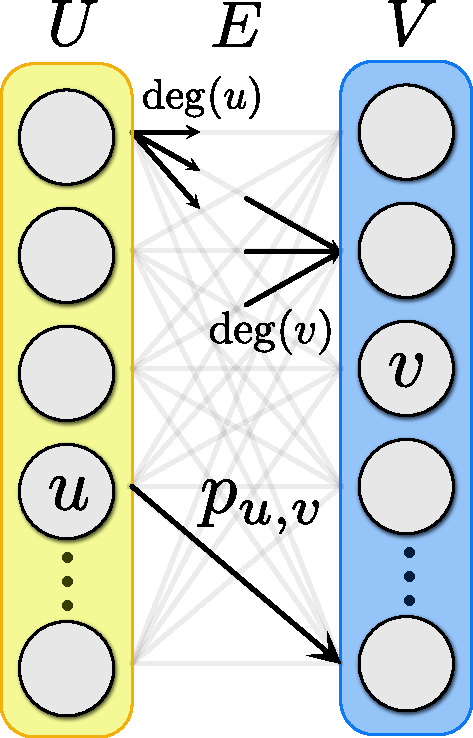
\includegraphics[width=0.4\columnwidth]{figures/bipartite_map.pdf}
	\caption{\textbf{Swap symmetry.}???.}\label{fig:swap_symmetry}
\end{figure}

* Space of satisfying graph assignments is given by the action of the consensus group on any valid graph assignment,
\begin{align}
	\{\mathcal{G}\} = C_d \times \mathcal{G}_{n,d}.
\end{align}


* Clarify edge transformations rather than U and V.

* Permutation group

* Graph automorphisms not the same as automorphisms over edges.

* Automorphism group in edge space describes invariances. Sym/Aut gives consensus group?

* Automorphism group over edge permutations is in general inequivalent to the conventional definition of a graph automorphism: for $\mathcal{G}=(V,E)$, $(u,v)\in E \Leftrightarrow (\sigma(u),\sigma(v))\in E$ %$\mathrm{Aut}(\mathcal{G}): $

* Counting graph automorphisms is known to be

* While all permutations within $E_U$ and $E_V$ are degree preserving, not all are unique.

Transformations over the space of satisfying graph realisations of given degree sequence, $d$, defines the \emph{consensus group}, $C(d)$, fully characterised by its degree sequence. Over the space of satisfying graphs the consensus group,
\begin{align}
	\phi: C(d)\times \mathcal{G}_d \to \mathcal{G}_d,
\end{align}
is identically the symmetric group,
\begin{align}
	\phi: C(d) = \mathrm{Sym}(\mathcal{G}_d).
\end{align}
The action of the consensus group may be equivalently defined via permutations within the columns of satisfying edge-sets,
\begin{align}
	\psi: C(d)\times (E_U\times E_V) \to (E_U\times E_V),
\end{align}
the group of non-degenerate permutations within the columns of $E$, which discounts permutations under which edge-sets remain invariant, a subgroup of the symmetric group acting on either column, both of length $|E|$,
\begin{align}
	(\psi, E_{U,V}) & \subseteq S_{|E|}.
\end{align}

In the special case of 1-regular graphs, satisfying consensus assignments define bijective maps across graph partitions and the group action over edge-set columns is identically the symmetric group,
\begin{align}
	\psi: C(d) = S_{|E|},\,\delta(\mathcal{G})=\Delta(\mathcal{G})=1,
\end{align}
as there are no degenerate permutations.

Hence, the order of the consensus group, equivalently the number of unique consensus assignments, is upper-bounded by the order of the symmetric group acting on edge-sets, $S_{|E|}$,
\begin{align} \label{eq:orbit_order}
	%|C(d)| &= \frac{|E|!}{\prod_{u\in U}\mathrm{deg}(u)!\cdot \prod_{v\in V}\mathrm{deg}(v)!} \nonumber\\
	%&= \binom{|E|!}{d_1,\dots,d_{|U|+|V|}} \nonumber\\
	|C(d)| & \leq |E|!,
\end{align}
with equality when \mbox{$\Delta(\mathcal{G})=1$}.

Employing element-wise inequality notation for degree sequences, of equal length, \mbox{$|d|=|d'|$},
\begin{align}
	d' < d \coloneqq d'_i < d_i,\, \forall\, i,
\end{align}
affords the equivalent relations between degree sequences, satisfying assignment graphs and their respective subgroup structures,
\begin{align} \label{eq:sub_dgc}
	d' < d & \Rightarrow \mathcal{G}_{d'} \subset \mathcal{G}_d \Rightarrow C(d') \triangleleft C(d),
\end{align}
where $C(d')$ is a normal subgroup of $C(d)$ and $\mathcal{G}_{d'}$ is a subgraph of $\mathcal{G}_d$ under edge-removal.

%Consensus groups exhibit a recursive normal subgroup structure,
%\begin{align}
%	C(d') &\triangleleft C(d),
%\end{align}
%reflecting the associated subgraph structure,
%\begin{align}
%	\mathcal{G}' &\subset \mathcal{G}.
%\end{align}

%As edge exchange operations are symmetric across $U$ and $V$ the consensus group may equivalently be associated with the space of edge permutations on either. Despite having support over vertex sets with distinct degree sequences they afford the same space of edge permutations.

The number of bits required to uniquely address the group's orbit scales as (Fig.~\ref{fig:bits_permutations}),
\begin{align}
	n & = \log_2(|\mathrm{Orb}_C(E)|) \leq \log_2(|E|!).
\end{align}

\begin{figure}[!htb]
	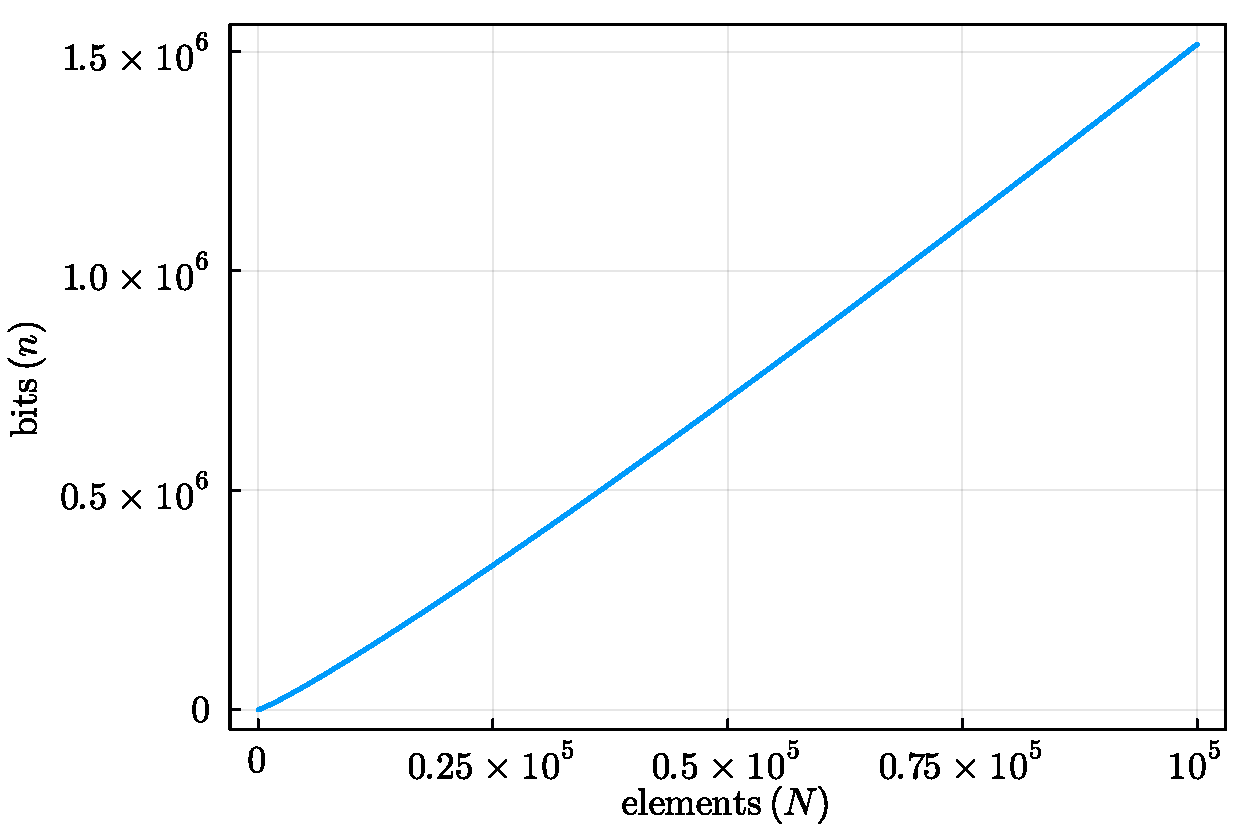
\includegraphics[width=\columnwidth]{figures/bits_permutations.pdf}
	\caption{\textbf{Number of bits ($n$) required to encode an arbitrary permutation ($S_N$) over $N$ elements.} This upper-bounds the required number of bits to uniquely address elements of the consensus group, $C(d)$.} \label{fig:bits_permutations}
\end{figure}

\subsection{Uniform consensus sampling} \label{sec:uniform_consensus_samp}

Secure consensus assignment requires assigning edge-sets uniformly at random over the space of all satisfying edge-sets. Uniformity implies maximisation of entropy, given by,
\begin{align}
	H(C(d)) = \log_2(|C(d)|),
\end{align}
where $|C(d)|$ is the order of the respective consensus group. Degeneracies in permutations result in sampling bias thereby reducing entropy, requiring that algorithmic implementation does not double-count degenerate permutations from the symmetric group.

\subsubsection{Fisher-Yates shuffle}

The Fisher-Yates shuffle \cite{FisherYates53} is an efficient algorithm for applying in-place permutations $\pi\in S_n$ to an array of $n$ elements uniformly at random (Alg.~\ref{alg:fisher_yates}).

The algorithm iteratively allows every array index to randomly exchange itself with any element not already assigned. Assuming $O(1)$ random number generation the Fisher-Yates shuffle exhibits $O(n)$ time-complexity. As the operational primitive is the exchange operation the algorithm permutes arrays in-place.

The sequence of $O(n)$ random numbers chosen during execution defines a decision tree whose $i$th level assigns the $i$th array index. Individual execution paths correspond to individual permutations with a one-to-one correspondence. Hence, the algorithm's execution space $\mathcal{L}_n$ is isomorphic to the symmetric group,
\begin{align}
	\mathcal{L}_n \cong S_n,
\end{align}
under mapping between execution paths \mbox{$l\in\mathcal{L}_n$} and permutations \mbox{$\pi\in S_n$}. As all execution paths occur with uniform probability $1/n!$ the algorithm uniformly samples from the symmetric group.

\begin{algorithm}[H]
	\begin{algorithmic}
		\Function{FisherYatesShuffle}{$\vec{v}$} $\to \vec{v}$ \Comment{$O(n)$}
		\For{$i \gets |\vec{v}|-1 \textbf{ to } 1$} \Comment{$O(n)$}
		\State $j \gets \textsc{Random}(\{0,\dots,i\})$ \Comment{$O(1)$}
		\State $v_i\leftrightarrow v_j$ \Comment{Exchange}
		\EndFor
		\State \Return $\vec{v}$
		\EndFunction
	\end{algorithmic}
	\caption{\cite{FisherYates53} The Fisher-Yates shuffle algorithm for applying a random permutation $\pi\in S_{|\vec{v}|}$ to the elements a vector $\vec{v}$. The algorithm permutes  vectors in-place with $O(n)$ runtime assuming an $O(1)$ \textsc{Random}($\cdot$) function.}\label{alg:fisher_yates}
\end{algorithm}

The uniqueness of execution paths may be seen by noting that an element at index $j\leq i$ has  exactly one path to be reassigned to index $i$, via the direct exchange $v_i\leftrightarrow v_j$ when the loop reaches index $i$.

The execution path $l\in\mathcal{L}_n$ of the algorithm directly relates to the cycle decomposition of the respective group element. As the algorithm iterates through $i$ the series of exchange operations defines a path. When a trivial $v_i\leftrightarrow v_i$ exchange occurs it terminates that path, closing it as a cycle, after which the next $i$ opens a new one.

Closely related to the Fisher-Yates shuffle is Sattolo's algorithm \cite{Sattolo86} for uniformly sampling the cyclic group ($C_n$) differing only from the Fisher-Yates shuffle in the set of allowed exchanges,
\begin{align}
	\text{Fisher-Yates }(S_n):\,\, & 0\leq j\leq i,\nonumber \\
	\text{Sattolo }(C_n):\,\,      & 0\leq j<i.
\end{align}
Note that this distinction serves to prohibit trivial exchanges ($v_i\leftrightarrow v_i$) thereby forcing all execution paths to define single cycles.

\subsubsection{Generalised Fisher-Yates shuffle for finite groups}

The Fisher-Yates shuffle may be generalised to uniformly sample over other finite groups (Alg.~\ref{alg:fisher_yates_general}).

Alg.~\ref{alg:fisher_yates} may be interpreted as follows: for every index $i$ the associated value $v_i$ is chosen uniformly from the set of unassigned values $v_j$ (where $0\leq j\leq i$). More generally, we would choose $v_i$ uniformly from the set of elements it is allowed to transition to under the action of the respective group. For the symmetric group, $S_n$, this includes all elements, whereas other groups in general constrain the set of allowed transitions.

Consider a group $G$ defined over set $X$,
\begin{align}
	\phi: G\times X \to X.
\end{align}
Elements of the set $x\in X$ individually transform under the group action of $G$ to their orbit,
\begin{align}
	\mathrm{Orb}_G(x) & = G\times x \nonumber                                         \\
	                  & = \{ y\in X \,\,|\,\, \exists \,g\in G \,\,|\,\, y=g\cdot x\}
\end{align}
defining sets for the allowed transitions of $x$ under the action of $G$. For the symmetric group we have,
\begin{align}
	\mathrm{Orb}_{S_n}(x) = X,
\end{align}
as all elements may map to all others, while for other groups the orbit of $x$ may be a subset of elements.

We define the \emph{transition set}, $t$, to be the set of allowed transitions of $x$ under the group action of $G$, given by the intersection unassigned elements ($s$) and the orbit of $x$,
\begin{align}
	t = \mathrm{Orb}_G(x) \cap s.
\end{align}

%Sattolo's algorithm for uniformly sampling the cyclic group defines the transition set to include all unassigned elements excluding element $i$. This arises because under a cyclic permutation all elements must permute

\begin{algorithm}[H]
	\begin{algorithmic}
		\Function{GroupShuffle}{$\vec{v}$, $G$} $\to \vec{v}$\Comment{$O(n^2)$}
		\For{$i \gets |\vec{v}|-1 \textbf{ to } 1$} \Comment{$O(n)$}
		\State $s \gets \{\vec{v}_j\,|\, 0\leq j\leq i\}$ \Comment{Unassigned elements}
		\State $t \gets \textsc{TransitionSet}(\vec{v}_i,s,G)$ \Comment{$O(n)$}
		\State $j \gets \textsc{Random}(t)$ \Comment{$O(1)$}
		\State $v_i\leftrightarrow v_j$ \Comment{Exchange}
		\EndFor
		\State \Return $\vec{v}$
		\EndFunction
		\\
		\Function{TransitionSet}{$x$, $s$, $G$} $\to t$ \Comment{$O(n)$}
		\State \Return $(G\times x) \cap s$ \Comment{Group action on reduced set}
		\EndFunction
	\end{algorithmic}
	\caption{Generalised Fisher-Yates shuffle for finite groups $G$.}\label{alg:fisher_yates_general}
\end{algorithm}

\textbf{WRONG FOR THE CONSENSUS GROUP:} The uniqueness of execution paths in the generalised algorithm follows the same argument as for the the original scheme. The probability associated with an execution path is,
\begin{align} \label{eq:group_order_shuffle}
	P(\vec{d}) & = \prod_{i=1}^{n} p(\vec{d}_i) = \prod_{i=1}^{n} \frac{1}{|t_i|} = \prod_{i=1}^{n} \frac{1}{|\mathrm{Orb}_{G^{(i)}}(x_i)|},
\end{align}
where \mbox{$\vec{d}_i=1/|t_i|$} is the probability of making choice \mbox{$j=\vec{d}_i$} at level $i$ under uniform sampling, and $G^{(i)}$ denotes the $i$th level subgroup of $G=G^{(n)}$ acting on the reduced set predicated on the removal of already assigned elements of $X$,
\begin{align} \label{eq:subgroup_struct}
	G^{(i)}   & \times X^{(i)} \to X^{(i)},\nonumber   \\
	X^{(i)}   & = X\backslash\{x_{k}\}_{k>i},\nonumber \\
	G^{(i-1)} & \triangleleft G^{(i)},
\end{align}
defining a composition series followed by the algorithm to iteratively assign set elements,
\begin{align}
	1 = G^{(0)} \triangleleft \cdots \triangleleft G^{(n-1)} \triangleleft G^{(n)} = G,
\end{align}
where each subgroup acts on the set predicated on the removal of an element from the set upon which the supergroup acts.

As the consensus group is both free\footnote{Free groups: all elements are invariant under the action of all group elements except the identity,
	\begin{align}
		g\cdot x = x\, \Rightarrow\, g=e.\nonumber
	\end{align}} and transitive\footnote{Transitive groups: all elements $x\in X$ map to all elements $y\in X$ under the action of some group element $g\in G$,
	\begin{align}
		x,y\in X \,|\, \exists\, g\in G \,\,|\,\, g\cdot x=y.\nonumber
	\end{align}}
it has regular\footnote{Regular group action: $\forall\,\,x,y\in X \,\,|\,\, g\cdot x=y$, $g\in G$ is unique.} group action and all group elements have the same orbit. Hence, $|t_i|$ is level-dependent on $i$ but independent of group element $x\in X$ and execution pathway $l\in\mathcal{L}$. $P(\vec{d})$ is therefore a function of the group but uniform across all group elements.

\subsubsection{Uniformly sampling the consensus group}

Uniformly sampling the consensus group is achieved by defining transition sets as per Alg.~\ref{alg:consensus_shuffle}, whereby allowed transitions under edge exchanges \mbox{$v_i\leftrightarrow v_j$} satisfy the Boolean constraint,
\begin{align}
	[(u_i,v_j) \not\in E] \lor [(u_j,v_i)	\not\in E] = 1,
\end{align}
requiring that newly created edges not be previously existing ones. ??? CHECK

An \mbox{$v_i\leftrightarrow v_j$} exchange within edge-set $E$ is equivalent to eliminating existing edges,
\begin{align}
	e_i = (u_i,v_i),\,\, e_j = (u_j,v_j),
\end{align}
and replacing them with permuted edges,
\begin{align}
	e_i' = (u_i,v_j),\,\, e_j' = (u_j,v_i).
\end{align}
Thus, edge-set invariance under \mbox{$v_i\leftrightarrow v_j$} requires,
\begin{align}
	E \backslash \{e_i,e_j\} \cup \{e_i',e_j'\} = E,
\end{align}
which implies,
\begin{align}
	\{e_i',e_j'\}            & \in E,\nonumber                        \\
	E \backslash \{e_i,e_j\} & = E \backslash \{e_i',e_j'\},\nonumber \\
	\{e_i,e_j\}              & =\{e_i',e_j'\}.
\end{align}
Hence, the requirement exchanges \mbox{$v_i\leftrightarrow v_j$} not be edge-set invariant is,
\begin{align}
	\{e_i',e_j'\}            & \in E,\nonumber                        \\
	E \backslash \{e_i,e_j\} & = E \backslash \{e_i',e_j'\},\nonumber \\
	\{e_i,e_j\}              & =\{e_i',e_j'\}.
\end{align}

%\begin{align}
%	E \backslash \{e_i,e_j\} = E \backslash \{e_i',e_j'\}.
%\end{align}

%As the edge-sets of simple graphs are simple sets, 

%
%* The exchange operation $v_i\leftrightarrow v_j$ prospectively creates the new edges $(u_i,v_j)$ and $(u_j,v_i)$. If either already exist this would either: violate $\mathcal{G}$ being a simple graph; constitute a degenerate edge permutation. Hence, 

* Need to clarify notation here. $i$ here refers to index in $E$, but usually we use it for a node number.

%\begin{align} \label{eq:exchange_rule}
%		(u_i \neq u_j) \odot (v_i \neq v_j) = 1,
%\end{align}
%where $\odot$ denotes logical XNOR. This constraint is equivalent to,
%\begin{align}
%		[(u_i \neq u_j) \land (v_i \neq v_j)] \lor [(u_i = u_j) \land (v_i = v_j)] = 1,
%\end{align}
%where the first clause allows exchange operations between nodes $u_i$ and $u_j$, equivalently between consensus sets $v_i$ and $v_j$, only when distinct (Fig.~\ref{fig:swap_sym}), and the second clause is equivalent to $i=j$, ensuring inclusion of $u_i$ itself.

%\begin{figure}[!htb]
%\centering
%\begin{tikzpicture}[genericStyle, every node/.style={circle, draw, minimum size=1.7em, text width=1em, align=center, inner sep=0pt}]
    \def\UVsep{2.5em}
    \def\colSep{3em}
    \def\rowSep{1.2em}
    \def\hStep{0.7em}

    % Figure 1
    \node[nodeUStyle] (a1) at (0,0) {$u_i$};
    \node[nodeUStyle] (a2) [below=\hStep of a1] {$u_j$};
    \node[nodeVStyle, right=\UVsep of a1] (b1) {$v_i$};
    \node[nodeVStyle, right=\UVsep of a2] (b2) {$v_j$};

    \draw[graphEdgeStyle] (a1) -- (b1); 
    \draw[graphEdgeStyle] (a2) -- (b2);

    \coordinate (midA) at ($(a1.south)!0.5!(a2.north)$);
    \node[draw=none, left=0.4em of midA]
    {$\Big\updownarrow$};

    \node[nodeUStyle, right=\colSep of b1] (c1) {$u_i$};
    \node[nodeUStyle, right=\colSep of b2] (c2) {$u_j$};
    \node[nodeVStyle, right=\UVsep of c1] (d1) {$v_i$};
    \node[nodeVStyle, right=\UVsep of c2] (d2) {$v_j$};

    \draw[graphEdgeStyle] (c1) -- (d2); 
    \draw[graphEdgeStyle] (c2) -- (d1);

    \coordinate (midB) at ($(b1.east)!0.5!(b2.east)$); 
    \coordinate (midC) at ($(c1.west)!0.5!(c2.west)$);
    \coordinate (midBC) at ($(midB)!0.5!(midC)$);
    \node[draw=none, text width=2em] at (midBC) {$\Longleftrightarrow$};  

    % Figure 2
    \node[nodeUStyle] (a3) [below=\rowSep of a2] {};
    \node[nodeUStyle] (a4) [below=\hStep of a3] {};

    \coordinate (midA2) at ($(a3.south)!0.5!(a4.north)$);
    \node[draw=none, left=0.4em of midA2]
    {$\Big\updownarrow$};

    \coordinate (midA3) at ($(a3.east)!0.5!(a4.east)$);
    \node[nodeVStyle, right=\UVsep of midA3] (b3) {};
    \draw[graphEdgeStyle] (a3) -- (b3);
    \draw[graphEdgeStyle] (a4) -- (b3);

    \node[nodeUStyle, below=\rowSep of c2] (c3) {};
    \node[nodeUStyle, below=\hStep of c3] (c4) {};

    \coordinate (midC3) at ($(c3.east)!0.5!(c4.east)$);
    \node[nodeVStyle, right=\UVsep of midC3] (d3) {};
    \draw[graphEdgeStyle] (c3) -- (d3);
    \draw[graphEdgeStyle] (c4) -- (d3);

    \coordinate (midC2) at ($(c3.west)!0.5!(c4.west)$);
    \coordinate (midBC2) at ($(b3.east)!0.5!(midC2)$);
    \node[draw=none, text width=2em] at (midBC2) {$\Longleftrightarrow$};  
\end{tikzpicture}

%%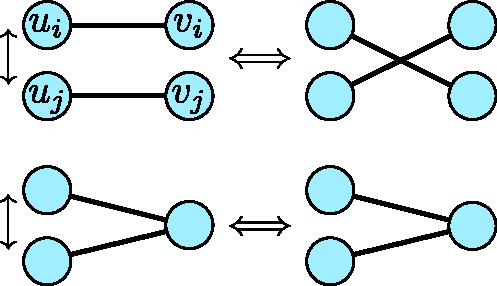
\includegraphics[width=0.5\columnwidth]{figures/swap_symmetry.pdf}
%\caption{\textbf{Degeneracy rule for vertex exchanges in the consensus group.} Allowed vertex exchanges $u_i\leftrightarrow u_j$ (equivalently $v_i\leftrightarrow v_j$) require vertices in both the $U$ and $V$ partitions of the bipartite graph to be distinct, as per Eq.~\eqref{eq:exchange_rule}.} \label{fig:swap_sym}	
%\end{figure}

\begin{algorithm}[H]
	\begin{algorithmic}
		\Function{ConsensusShuffle}{$\mathcal{X}$, $\vec{u}$, $\vec{v}$} $\to \vec{v}$ \Comment{$O(n^2)$}
		\For{$i \gets |\vec{v}|-1 \textbf{ to } 1$} \Comment{$O(n)$}
		\State $t \gets \{0\leq k< i \,|\, \textsc{Transition}(i,k) = 1\}$ \Comment{$O(n)$}
		\State $j \gets \textsc{Random}(\mathcal{X}, t \cup i)$ \Comment{$O(1)$}
		\State $v_i\leftrightarrow v_j$ \Comment{Exchange}
		\EndFor
		\State \Return $\vec{v}$
		\EndFunction
		\\
		\Function{AllowTransition}{$i$, $j$} $\to \{0,1\}$ \Comment{$O(n)$}
		\State \Return $[(u_i,v_j) \notin E] \land [(u_j,v_i) \notin E]$
		\EndFunction
	\end{algorithmic}
	\caption{The transition set for the consensus group may be characterised by the constraints imposed by the group relations characterising non-degenerate transitions. The \textsc{Transition} function is a binary operator specifying whether index $j$ is an allowed transition for index $i$, defining the respective transition set.}\label{alg:consensus_shuffle}
\end{algorithm}

The regular action of the consensus group implies that under symmetrisation via uniform sampling all satisfying edge assignments $\{E\}$ occur with equal probability, from which it follows,
% It follows that every node $u$ will be ass, and nodes are assigned with uniform probability to all consensus sets, and every consensus set has uniform probability of comprising any subset of nodes,
\begin{align} \label{eq:prob_cons}
	p_{u,v}                       & = \frac{\mathrm{deg}(u)}{|V|},\nonumber \\
	\sum_{v\in V} p_{u,v}         & = \mathrm{deg}(u),\nonumber             \\
	\sum_{u\in U} p_{u,v}         & = 1, \nonumber                          \\
	\sum_{u\in U, v\in V} p_{u,v} & = |E|,
\end{align}
where $p_{u,v}$ is the probability of node $u$ being assigned to consensus set $v$.
* Regular action.

* Use uniform bidding to preserve average case $r$. If non-uniform the effective $r$ in consensus sets is biased towards the $r$ of higher bidders.

* ???
* For a given edge $e=(u,v)$ in edge-set $e\in E$, the order of the orbit of vertex $v$ under the group action $\psi$ is,
\begin{align}
	\psi: |\mathrm{Orb}_C(v)| & = |V/v| = |V|-1.
\end{align}
That is, vertex $v$ may permute to any vertex other than itself.

* ??? TODO. Fig.~\ref{fig:bipartite_map}

* Bipartite decomposition or bipartite dimension. Edge-disjoint union of complete bipartite graphs or bicliques.

* Degree-preserving biclique decomposition.

* Kmn defines invariant subgraphs under edge-permutation. Vertices within a Kmn subgraph define graph automorphisms under vertex permutations $\sigma$.
\begin{align}
	\varphi: (u,v)\in E \Longleftrightarrow (\sigma_u,\sigma_v)	\in E.
\end{align}

For complete graphs all vertex permutations within each bipartition define graph automorphisms,
\begin{align}
	\mathrm{Aut}(K_{m,n}) = S_m\times S_n.
\end{align}


* Graph sum (disjoint union)
\begin{align}
	\mathcal{G}_d^{(K)} = \bigoplus_{b} K_{m_b,n_b}.
\end{align}

* Not all graphs can be decomposed this way. Determining this is NP-hard in general.

For $K_{m,n}$,
\begin{align}
	\mathrm{deg}(u) & =n,\,\forall\, u\in U,\nonumber \\
	\mathrm{deg}(v) & =m,\,\forall\, v\in V.
\end{align}

* Admits graph automorphisms,
\begin{align}
	\bigtimes_{b} (S_{m_b}\times S_{n_b}) \subseteq \mathrm{Aut}(\mathcal{G}_d^{(K)}).
\end{align}
* Is it equality?

\begin{figure}[!htb]
	\begin{tikzpicture}[genericStyle]
    \def\Km{5}
    \def\Kn{4}
    \def\Kmskip{4}
    \def\Knskip{3}
    \def\voff{-0.575}
    \def\dotsoff{0.15}
    \def\UVsep{2.8}
    
    \foreach \i in {1,...,\Km} {
        \ifnum\i=\Kmskip
          \node[draw=none] (a\i) at (0,\dotsoff-\i) {\LARGE $\vdots$};
        \else
            \ifnum\i=\Km
                \node[nodeUStyle] (a\i) at (0,-\i) {$u_m$};
            \else
                \node[nodeUStyle] (a\i) at (0,-\i) {$u_{\i}$};
            \fi
        \fi
    }
    \foreach \i in {1,...,\Kn} {
        \ifnum\i=\Knskip
            \node[draw=none] (b\i) at (\UVsep,\dotsoff+\voff-\i) {\LARGE $\vdots$};
        \else
            \ifnum\i=\Kn
                \node[nodeVStyle] (b\i) at (\UVsep,\voff-\i) {$v_n$};
            \else
                \node[nodeVStyle] (b\i) at (\UVsep,\voff-\i) {$v_{\i}$};
            \fi
        \fi
    }
    
    \foreach \i in {1,...,\Km} {
        \foreach \j in {1,...,\Kn} {
        \ifnum\i=\Kmskip
        \else
            \ifnum\j=\Knskip
            \else
                \draw[graphEdgeStyle] ($(a\i.east)$) -- ($(b\j.west)$);
            \fi
        \fi
        }
    }

    \node[draw=none] at ($(a1)!0.5!(b1) + (0,0.5)$) {$K_{m,n}$};
\end{tikzpicture}
	\caption{\textbf{Complete bipartite graph, $K_{m,n}$.} Vertices in each bipartition have uniform degree.} \label{fig:K_mn_graph}
\end{figure}

\begin{figure}[!htb]
	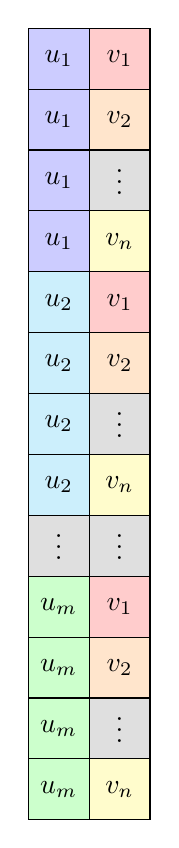
\begin{tikzpicture}
  \tikzset{square node/.style={draw, minimum size=2.2em}}

    \definecolor{verylightgray}{rgb}{0.9, 0.9, 0.9}
    \colorlet{color1}{blue!20}
    \colorlet{color2}{cyan!20}
    \colorlet{color3}{green!20}

    \colorlet{colorA}{red!20}
    \colorlet{colorB}{orange!20}
    \colorlet{colorC}{yellow!20}

  \def\x{2.2em}

    % 1
    \node[square node, fill=color1] at (\x,-\x) {$u_1$};
    \node[square node, fill=colorA] at (2*\x,-\x) {$v_1$};

    \node[square node, fill=color1] at (\x,-2*\x) {$u_1$};
    \node[square node, fill=colorB] at (2*\x,-2*\x) {$v_2$};
    
    \node[square node, fill=color1] at (\x,-3*\x) {$u_1$};
    \node[square node, fill=lightgray!50] (d1) at (2*\x,-3*\x) {};
    \node[draw=none] at (d1) [yshift=0.25em] {$\vdots$};

    \node[square node, fill=color1] at (\x,-4*\x) {$u_1$};
    \node[square node, fill=colorC] at (2*\x,-4*\x) {$v_n$};

     % 2
    \node[square node, fill=color2] at (\x,-5*\x) {$u_2$};
    \node[square node, fill=colorA] at (2*\x,-5*\x) {$v_1$};

    \node[square node, fill=color2] at (\x,-6*\x) {$u_2$};
    \node[square node, fill=colorB] at (2*\x,-6*\x) {$v_2$};
    
    \node[square node, fill=color2] at (\x,-7*\x) {$u_2$};
    \node[square node, fill=lightgray!50] (d2) at (2*\x,-7*\x) {};
    \node[draw=none] at (d2) [yshift=0.25em] {$\vdots$};

    \node[square node, fill=color2] at (\x,-8*\x) {$u_2$};
    \node[square node, fill=colorC] at (2*\x,-8*\x) {$v_n$};

    % ...
    \node[square node, fill=lightgray!50] (d3) at (\x,-9*\x) {};
    \node[draw=none] at (d3) [yshift=0.25em] {$\vdots$};
    \node[square node, fill=lightgray!50] (d4) at (2*\x,-9*\x) {};
    \node[draw=none] at (d4) [yshift=0.25em] {$\vdots$};

    % m
    \node[square node, fill=color3] at (\x,-10*\x) {$u_m$};
    \node[square node, fill=colorA] at (2*\x,-10*\x) {$v_1$};

    \node[square node, fill=color3] at (\x,-11*\x) {$u_m$};
    \node[square node, fill=colorB] at (2*\x,-11*\x) {$v_2$};
    
    \node[square node, fill=color3] at (\x,-12*\x) {$u_m$};
    \node[square node, fill=lightgray!50] (d5) at (2*\x,-12*\x) {};
    \node[draw=none] at (d5) [yshift=0.25em] {$\vdots$};

    \node[square node, fill=color3] at (\x,-13*\x) {$u_m$};
    \node[square node, fill=colorC] at (2*\x,-13*\x) {$v_n$};

\end{tikzpicture}
	\caption{\textbf{Canonically ordered edge-set for complete bipartite graph, $K_{m,n}$.}} \label{fig:K_mn_edges}
\end{figure}

\begin{figure}[!htb]
\centering
	\begin{minipage}[t]{0.4\columnwidth}
		\begin{tikzpicture}[genericStyle]
    \def\UVsep{2.5}
    \def\vMult{1.8}
    
    \colorlet{color1}{blue}
    \colorlet{color2}{cyan}
    \colorlet{color3}{green}
    \colorlet{colorA}{red}
    \colorlet{colorB}{orange}
    \colorlet{colorC}{yellow}
    
    \node[draw=color1, fill=color1!20, myShadow] (a1) at (0,-1*\vMult) {$u_1$};
    \node[draw=color2, fill=color2!20, myShadow] (a2) at (0,-2*\vMult) {$u_2$};
    \node[draw=color3, fill=color3!20, myShadow] (a3) at (0,-3*\vMult) {$u_3$};
    
    \node[draw=colorA, fill=colorA!20, myShadow] (b1) at (\UVsep,-1*\vMult) {$v_1$};
    \node[draw=colorB, fill=colorB!20, myShadow] (b2) at (\UVsep,-2*\vMult) {$v_2$};
    \node[draw=colorC, fill=colorC!20, myShadow] (b3) at (\UVsep,-3*\vMult) {$v_3$};
    
     \foreach \i in {1,...,3} {
     	\foreach \j in {1,...,3} {
        	\draw[graphNonEdgeStyle] ($(a\i.east)$) -- ($(b\j.west)$);
        }
    }
    
    \draw[graphEdgeStyle] ($(a1.east)$) -- ($(b1.west)$);
    \draw[graphEdgeStyle] ($(a1.east)$) -- ($(b2.west)$);
    \draw[graphEdgeStyle] ($(a2.east)$) -- ($(b2.west)$);
    \draw[graphEdgeStyle] ($(a2.east)$) -- ($(b3.west)$);
    \draw[graphEdgeStyle] ($(a3.east)$) -- ($(b3.west)$);
    \draw[graphEdgeStyle] ($(a3.east)$) -- ($(b1.west)$);
    
    \node[draw=none] at ($(a1)!0.5!(b1) + (0,0.75)$) {$\mathcal{G}_{3,2}$};
\end{tikzpicture}
	\end{minipage}
	\quad
	\begin{minipage}[t]{0.3\columnwidth}
		\begin{tikzpicture}
  \tikzset{square node/.style={draw, minimum size=2.2em}}
  \colorlet{color1}{blue}
  \colorlet{color2}{cyan}
  \colorlet{color3}{green}

  \colorlet{colorA}{red}
  \colorlet{colorB}{orange}
  \colorlet{colorC}{yellow}

  \def\x{2.2em}

  \node[square node, fill=color1!20] (u1) at (\x,-\x) {$u_1$};
  \node[square node, fill=colorA!20] (v1) at (2*\x,-\x) {$v_1$};
  \node[square node, fill=color1!20] at (\x,-2*\x) {$u_1$};
  \node[square node, fill=colorB!20] at (2*\x,-2*\x) {$v_2$};

  \node[square node, fill=color2!20] at (\x,-3*\x) {$u_2$};
  \node[square node, fill=colorB!20] at (2*\x,-3*\x) {$v_2$};
  \node[square node, fill=color2!20] at (\x,-4*\x) {$u_2$};
  \node[square node, fill=colorC!20] at (2*\x,-4*\x) {$v_3$};

  \node[square node, fill=color3!20] at (\x,-5*\x) {$u_3$};
  \node[square node, fill=colorC!20] at (2*\x,-5*\x) {$v_3$};
  \node[square node, fill=color3!20] at (\x,-6*\x) {$u_3$};
  \node[square node, fill=colorA!20] at (2*\x,-6*\x) {$v_1$};

  \node[draw=none] at ($(u1)!0.5!(v1) + (0,0.75)$) {$E$};
\end{tikzpicture}
	\end{minipage}
	\caption{\textbf{Consensus assignment graph ($\mathcal{G}_{3,2}$) and its respective edge-set ($E$).}} \label{fig:G_32_edges}
\end{figure}

\subsubsection{Counting bipartite graph realisations} \label{sec:count_real}

The structure of the \textsc{ConsensusShuffle} algorithm (Alg.~\ref{alg:consensus_shuffle}) via Eq.~\eqref{eq:group_order_shuffle} affords evaluation of the order of the consensus group equivalently counting bipartite graph realisations for a given degree sequence,
\begin{align}
	|C(d)| = |\mathcal{G}_d|.
\end{align}

* The regular action of $C(d)$ affords the freedom to As all execution paths $l\in\mathcal{L}$

%Considering the $l_0\in\mathcal{L}$ execution path of Alg.~\ref{alg:consensus_shuffle}, corresponding to the identity group element $I \in C(d)$, during which no exchange operations take place, execution proceeds by iteratively eliminating the leading element of the ordered edge-set, with remaining edges unaffected, yielding the subgraph relation,
%\begin{align}
%	\mathcal{G}(\vec{E}\backslash\vec{E}_1) &\subset \mathcal{G}(\vec{E})
%\end{align}
%
%Assuming initial canonical graph assignment and sorted degree sequence (Alg.~\ref{alg:initial_assignment}), leading edge-removal equates to canonical graph assignment of the transformed degree sequence,
%\begin{align}
%	(d_U,d_V) \xrightarrow{\vec{E}\backslash\vec{E}_1} (\textsc{RedDeg}(d_U),\textsc{RedDeg}(d_V)),
%\end{align}
%where \textsc{RedDeg}($d$) decrements the leading element of $d$, truncated upon reaching zero, preserving initial ordering (Alg.~\ref{alg:count_bipartite}).
%
% which must not already belong to $E$.
%
%* Number of prohibited terms:



%* Let $d_U$ and $d_V$ denote the degree sequences for graph partitions $U$ and $V$, initially assumed to be normally ordered (decreasing by degree).

%* Assume input $E$ is in canonical form.

%* As the group action $G$ is regular we may equivalently choose any execution path and choose the identity path $l=I$ where no swaps take place under the group shuffle algorithm.

%* Acting on edge-set $E$ with leading element $e$ GroupShuffle implements:
%\begin{align}
%	|t_i(\mathrm{deg}(U),\mathrm{deg}(V)| &= |E| + 2 - d^{U}_1 - d^{V}_1 \nonumber\\
%	d^{U}_1 &= DecrementLeadDeg = d^{U}_1 - 1,\nonumber\\
%	d^{V}_1 &= d^{V}_1 - 1,\nonumber\\
%	(d^U,d^V) &= (\textsc{Trim}(d^U), \textsc{Trim}(d^V)),\nonumber\\
%	E &= E \backslash E_1 = \textsc{CanonicalGraph}(d^U,d^V),\nonumber\\
%	|E| &\to |E|-1,\nonumber\\
%\end{align}
%* Define reduced leading degree function \textsc{RLD}($d$,$i$) that subtracts a total of $i$ from vector $d$, starting at the first element, moving onto the next element when the current one reaches $0$, returning the first non-zero element of the reduced vector,
%following the convention of Eq.~\eqref{eq:subgroup_struct}. 
%* The order of the group $G$ acting on set $X$ is,
%\begin{align}
%	|C(d)| &= \prod_{i=1}^{|E|} |t_i(d)|,\\
%|t_i(d)| &= (|E|+3-i)\nonumber\\
%&-\sum_{j=1}^{\textsc{RLD}(d_U,i-1)}\mathrm{deg}(\textsc{RLD}(d_U,i-1)_j) \nonumber\\
%&-\sum_{j=1}^{\textsc{RLD}(d_V,i-1)}\mathrm{deg}(\textsc{RLD}(d_V,i-1)_j).\nonumber
%\end{align}

\begin{algorithm}[H]
	\begin{algorithmic}
		\Function{CountBipartiteReal}{$d$} $\to N$
		\State $d \gets \textsc{DegSort}(d)$ 	\State $N \gets 1$ \Comment{Group orbit size}
		\For{$i \gets 1 \textbf{ to } |E|$} \Comment{$O(|U|\cdot |V|)$}
		\State $t \gets \{0\leq k< i \,|\, \textsc{Transition}(i,k) = 1\}$ \Comment{$O(n)$}
		\State $N \gets N\cdot |t|$
		\EndFor
		\State \Return $N$
		\EndFunction
		\State
		%\Function{\textsc{TransitionSpace}}{$d$} $\to N$
		%	\State $|E| = \frac{1}{2}\sum_{i=1}d_i$
		%	\State $N \gets |E|+i-1$
		%	\State $t_U \gets \sum_{j=1}^{{d_U}'(1)} d_U'(j)$
		%	\State $t_V \gets \sum_{j=1}^{{d_V}'(1)} d_V'(j)$
		%	\State $N = \max(t_U,t_V)$
		%	\State \Return $N$
		%\EndFunction
		%\State
		%\Function{\textsc{RedDeg}}{$d$} $\to d$ \Comment{$O(1)$}
		%	\State $d_1 \gets d_1-1$ \Comment{Decrement leading degree}
		%		\If{$d_1=0$}
		%			\State $d \gets d_{2:|d|}$ \Comment{Truncate leading zeros}
		%		\EndIf
		%	\State \Return $d$ \Comment{Reduced}
		%\EndFunction
	\end{algorithmic}
	\caption{Count satisfying bipartite graph realisations for degree sequence $d$. \textsc{RedDeg}($d$) does not re-sort $d$, preserving its initial ordering. The elimination of zero-valued elements from $d$ equates to relabelling, but does not change the respective graph strcuture.} \label{alg:count_bipartite}
\end{algorithm}

%For 1-regular graphs we have,
%\begin{align}
%	d &= (1,\dots,1), \nonumber\\
%	\textsc{RLD}(d,i) &= 1,\,\forall\,i \nonumber\\
%	|t_i(d)| &= |E|+1-i,\nonumber\\
%	|C(d)| &= \prod_{i=1}^{|E|}(|E|+1-i)  =|E|!,
%\end{align}
%as expected for the symmetric group $S_{|E|}$.
%
%For complete bipartite graphs, $K_{m,n}$, we have,
%\begin{align}
%	d_U &= (n,\dots,n), \nonumber\\
%	d_V &= (m,\dots,m), \nonumber\\
%	RLD(d_U,i) &= n - (i\mod{n}),\nonumber\\
%	RLD(d_V,i) &= m - (i\mod{m}),\nonumber\\
%	|E| &= mn,\nonumber\\
%	|t_i(d)| &= (mn-m-n+3-i)\nonumber\\
%	&+(i\mod{n}) + (i\mod{m}).\nonumber
%\end{align}
%
%* Execution under identity operation:

\subsubsection{Sampling via random bitstreams} \label{sec:random_bitstreams}

As nodes must be in agreement on consensus assignment the \textsc{Random} functions relied upon during execution of Alg.~\ref{alg:consensus_shuffle} must evaluate consistently across network nodes, for which the established secure random bitstream $\mathcal{X}_\mathcal{N}$ (Sec.~\ref{sec:secure_shared_randomness}) is employed as per Alg.~\ref{alg:common_sampling}.

\begin{algorithm}[H]
	\begin{algorithmic}
		\Function{Random}{$\mathcal{X}$, $n$} $\to x$
		\Repeat
		\State $b \gets \lceil \log_2(n) \rceil$ \Comment{Minimum required number of bits}
		\State $x \gets \mathcal{X}.\mathtt{pop}(b)$ \Comment{Pop bits from bitstream}
		\Until{$x<n$} \Comment{Until $x$ is within bounds}
		\State \Return $x$
		\EndFunction
	\end{algorithmic}
	\caption{Deterministically choose an element $x$ from $n$ choices where $\mathcal{X}$ is a secure shared random bitstream. At most \mbox{$|\mathcal{X}| \leq \lceil \log_2(n) \rceil \cdot \log_2(1/\delta)$} bits are required to ensure success with probability \mbox{$p\geq 1-\delta$}.} \label{alg:common_sampling}
\end{algorithm}

While this function is deterministic it is not guaranteed to halt if $n\neq 2^b$ where $b\in\mathbb{Z}^+$. The success probability for a single iteration of the repeat block in Alg.~\ref{alg:common_sampling} is,
\begin{align}
	p_1(n) = \frac{n}{2^{\lceil \log_2(n) \rceil}} \geq \frac{1}{2},
\end{align}
where the worst-case lower-bound of $p=1/2$ arises when \mbox{$n=2^b+1$} for \mbox{$b\gg 1$},
\begin{align}
	p_1(2^b+1)                   & = \frac{1}{2} + \frac{1}{2^{b+1}},\nonumber \\
	\lim_{b\to\infty} p_1(2^b+1) & = \frac{1}{2}.
\end{align}
With $m$ rounds the success probability is,
\begin{align}
	p_m(n) = 1-(1-p_1)^m > 1-\frac{1}{2^m}.
\end{align}
Limiting the probability of failure to $\delta=1/2^m$ requires at most,
\begin{align}
	m \geq \log_2(1/\delta),
\end{align}
rounds. Hence, the worst-case consumption of random bits is,
\begin{align}
	|\mathcal{X}^{(n)}| \leq \lceil \log_2(n) \rceil \cdot \log_2(1/\delta).
\end{align}
The respective number of bits required to address all elements of the symmetric group, $S_n$, with $\delta$-likelihood of failure for all calls to \textsc{Random}$(\mathcal{X},\cdot)$ is,
\begin{align}
	|\mathcal{X}|^{(S_n)} & = \sum_{i=1}^n |\mathcal{X}^{(i)}| \nonumber                          \\
	                      & = \log_2(1/\delta) \cdot \sum_{i=1}^n \lceil\log_2(i)\rceil \nonumber \\
	                      & \approx \log_2(1/\delta) \cdot \log_2(n!),
\end{align}
an effective $\log_2(1/\delta)$ multiplicative overhead on the scaling relationship shown in Fig.~\ref{fig:bits_permutations}.

\subsubsection{Initial assignment} \label{sec:initial_graph_assignment}

\begin{figure}[!htb]
	\centering
	\begin{tikzpicture}[genericStyle]
    \def\N{10}
    \def\nskip{7}
    \def\conn{5}
    \def\UVsep{5}
    
    \foreach \i in {1,...,\N} {
        \ifnum\i=\nskip
          \node[draw=none] (a\i) at (0,-\i) {\LARGE $\vdots$};
        \else
            \ifnum\i=\N
                \node[nodeUStyle] (a\i) at (0,-\i) {}; % $u_m$
            \else
                \node[nodeUStyle] (a\i) at (0,-\i) {}; % $u_{\i}$
            \fi
        \fi
    }
    \foreach \i in {1,...,\N} {
        \ifnum\i=\nskip
            \node[draw=none] (b\i) at (\UVsep,-\i) {\LARGE $\vdots$};
        \else
            \ifnum\i=\N
                \node[nodeVStyle] (b\i) at (\UVsep,-\i) {}; % $v_n$
            \else
                \node[nodeVStyle] (b\i) at (\UVsep,-\i) {}; % $v_{\i}$
            \fi
        \fi
    }
    
     \foreach \i in {1,...,\N} {
     	\foreach \j in {1,...,\N} {
               \ifnum\i=\nskip
                \else
                	\ifnum\j=\nskip
                    \else
                        \draw[graphNonEdgeStyle] ($(a\i.east)$) -- ($(b\j.west)$);
                    \fi
                \fi
        }
    }

    
    \foreach \i in {1,...,\N} {
        \foreach \offset in {1,...,\conn} {
            \pgfmathtruncatemacro{\target}{mod(\i+\offset-2,\N)+1}
                \ifnum\i=\nskip
                \else
                \ifnum\target=\nskip
                    \else
                        \draw[graphEdgeStyle] ($(a\i.east)$) -- ($(b\target.west)$);
                    \fi
                \fi
        }
    }
    
  	\foreach \j in {1,...,\conn} {
                        \draw[-,redHighlightColor,line width=2,line cap=round] ($(a1.east)$) -- ($(b\j.west)$);
        }

    \node[draw=none] at ($(a1)!0.5!(b1) + (0,0.3)$) {$\mathcal{G}_{n,d}$};

    \coordinate (bracetop) at ($(b1.east) + (1em,0)$);
    \coordinate (bracetopin) at ($(bracetop) + (-0.1,0)$);
    \coordinate (bracebott) at ($(b\conn.east) + (1em,0)$);
    \coordinate (bracebottin) at ($(bracebott) + (-0.1,0)$);
    \draw[redHighlightColor, line width=1.5] (bracetopin) -- (bracetop) -- (bracebott) -- (bracebottin);

        \node[draw=none] at ($(bracetop)!0.5!(bracebott) + (3.5em,0)$) {$d=N(r/p,\varepsilon)$};
\end{tikzpicture}
	\caption{\textbf{Uniform bidding initial assignment graph.} \mbox{$\mathcal{G}_{n,d}$ has $n$ nodes and $n$ consensus sets, all with degree $d$.}}\label{fig:butterfly_graph}
\end{figure}

\begin{figure}[!htb]
	\centering
	\resizebox{0.31\columnwidth}{!}{
    \begin{tikzpicture}[genericStyle]
        \def\N{6}
        \def\nskip{8}
        \def\conn{1}
        \def\UVsep{2.8}

        \foreach \i in {1,...,\N} {
                \ifnum\i=\nskip
                    \node[draw=none] (a\i) at (0,-\i) {\LARGE $\vdots$};
                \else
                    \ifnum\i=\N
                        \node[nodeNetworkStyle] (a\i) at (0,-\i) {}; % $u_m$
                    \else
                        \node[nodeNetworkStyle] (a\i) at (0,-\i) {}; % $u_{\i}$
                    \fi
                \fi
            }
        \foreach \i in {1,...,\N} {
                \ifnum\i=\nskip
                    \node[draw=none] (b\i) at (\UVsep,-\i) {\LARGE $\vdots$};
                \else
                    \ifnum\i=\N
                        \node[nodeConsensusStyle] (b\i) at (\UVsep,-\i) {}; % $v_n$
                    \else
                        \node[nodeConsensusStyle] (b\i) at (\UVsep,-\i) {}; % $v_{\i}$
                    \fi
                \fi
            }


        \foreach \i in {1,...,\N} {
                \foreach \j in {1,...,\N} {
                        \ifnum\i=\nskip
                        \else
                            \ifnum\j=\nskip
                            \else
                                \draw[graphNonEdgeStyle] ($(a\i.east)$) -- ($(b\j.west)$);
                            \fi
                        \fi
                    }
            }

        \foreach \i in {1,...,\N} {
                \foreach \offset in {1,...,\conn} {
                        \pgfmathtruncatemacro{\target}{mod(\i+\offset-2,\N)+1}
                        \ifnum\i=\nskip
                        \else
                            \ifnum\target=\nskip
                            \else
                                \draw[graphEdgeStyle] ($(a\i.east)$) -- ($(b\target.west)$);
                            \fi
                        \fi
                    }
            }

        \node[draw=none] at ($(a1)!0.5!(b1) + (0,0.5)$) {\large $\mathcal{G}_{6,1}$};
    \end{tikzpicture}
}
	\hfill
	\resizebox{0.31\columnwidth}{!}{
\begin{tikzpicture}[genericStyle]
    \def\N{6}
    \def\nskip{8}
    \def\conn{3}
    \def\UVsep{2.8}
    
    \foreach \i in {1,...,\N} {
        \ifnum\i=\nskip
          \node[draw=none] (a\i) at (0,-\i) {\LARGE $\vdots$};
        \else
            \ifnum\i=\N
                \node[nodeUStyle] (a\i) at (0,-\i) {}; % $u_m$
            \else
                \node[nodeUStyle] (a\i) at (0,-\i) {}; % $u_{\i}$
            \fi
        \fi
    }
    \foreach \i in {1,...,\N} {
        \ifnum\i=\nskip
            \node[draw=none] (b\i) at (\UVsep,-\i) {\LARGE $\vdots$};
        \else
            \ifnum\i=\N
                \node[nodeVStyle] (b\i) at (\UVsep,-\i) {}; % $v_n$
            \else
                \node[nodeVStyle] (b\i) at (\UVsep,-\i) {}; % $v_{\i}$
            \fi
        \fi
    }
    
    
     \foreach \i in {1,...,\N} {
     	\foreach \j in {1,...,\N} {
               \ifnum\i=\nskip
                \else
                	\ifnum\j=\nskip
                    \else
                        \draw[graphNonEdgeStyle] ($(a\i.east)$) -- ($(b\j.west)$);
                    \fi
                \fi
        }
    }
    
    \foreach \i in {1,...,\N} {
        \foreach \offset in {1,...,\conn} {
            \pgfmathtruncatemacro{\target}{mod(\i+\offset-2,\N)+1}
                \ifnum\i=\nskip
                \else
                \ifnum\target=\nskip
                    \else
                        \draw[graphEdgeStyle] ($(a\i.east)$) -- ($(b\target.west)$);
                    \fi
                \fi
        }
    }

    \node[draw=none] at ($(a1)!0.5!(b1) + (0,0.5)$) {\large $\mathcal{G}_{6,3}$};
\end{tikzpicture}
}
	\hfill
	\resizebox{0.31\columnwidth}{!}{
\begin{tikzpicture}[genericStyle]
    \def\N{6}
    \def\nskip{8}
    \def\conn{6}
    \def\UVsep{2.8}
    
    \foreach \i in {1,...,\N} {
        \ifnum\i=\nskip
          \node[draw=none] (a\i) at (0,-\i) {\LARGE $\vdots$};
        \else
            \ifnum\i=\N
                \node[nodeUStyle] (a\i) at (0,-\i) {}; % $u_m$
            \else
                \node[nodeUStyle] (a\i) at (0,-\i) {}; % $u_{\i}$
            \fi
        \fi
    }
    \foreach \i in {1,...,\N} {
        \ifnum\i=\nskip
            \node[draw=none] (b\i) at (\UVsep,-\i) {\LARGE $\vdots$};
        \else
            \ifnum\i=\N
                \node[nodeVStyle] (b\i) at (\UVsep,-\i) {}; % $v_n$
            \else
                \node[nodeVStyle] (b\i) at (\UVsep,-\i) {}; % $v_{\i}$
            \fi
        \fi
    }
    
    
     \foreach \i in {1,...,\N} {
     	\foreach \j in {1,...,\N} {
               \ifnum\i=\nskip
                \else
                	\ifnum\j=\nskip
                    \else
                        \draw[graphNonEdgeStyle] ($(a\i.east)$) -- ($(b\j.west)$);
                    \fi
                \fi
        }
    }
    
    \foreach \i in {1,...,\N} {
        \foreach \offset in {1,...,\conn} {
            \pgfmathtruncatemacro{\target}{mod(\i+\offset-2,\N)+1}
                \ifnum\i=\nskip
                \else
                \ifnum\target=\nskip
                    \else
                        \draw[graphEdgeStyle] ($(a\i.east)$) -- ($(b\target.west)$);
                    \fi
                \fi
        }
    }

    \node[draw=none] at ($(a1)!0.5!(b1) + (0,0.5)$) {\large $\mathcal{G}_{6,6}=K_{6,6}$};
\end{tikzpicture}
}
	\caption{\textbf{Uniform bidding initial assignment graph.} \mbox{$\mathcal{G}_{n,d}$} has $n$ nodes and $n$ consensus sets, all with degree $d$, where \mbox{$d\leq n$}. For \mbox{$n=d$} we obtain the complete bipartite graph \mbox{$\mathcal{G}_{n,n}=K_{n,n}$.}}\label{fig:butterfly_graph_comp}
\end{figure}

Uniformly sampling consensus allocation requires applying sampled consensus group transformations (Alg.~\ref{alg:consensus_shuffle}) to an initial satisfying graph assignment (Fig.~\ref{fig:bipartite_map}) --- a solution to the \emph{bipartite realisation problem}. Via the Gale-Ryser theorem \cite{Gale1957, Ryser1957}, realisable bipartite graphs (those with \emph{bigraphic} degree sequences) demands,
\begin{align} \label{eq:bipartite_real}
	\sum_{i=1}^{|U|} \mathrm{deg}(u_i) & = \sum_{j=1}^{|V|} \mathrm{deg}(v_j),                                                     \\
	\sum_{i=1}^k \mathrm{deg}(u_i)     & \leq \sum_{j=1}^{|V|} \min(\mathrm{deg}(v_j),k),\,\forall\, k\in\{1,\dots,|V|\},\nonumber
\end{align}
where the second constraint assumes $U$ and $V$ are ordered decreasingly by degree. Realisable bipartite graphs may be efficiently realised using the Havel-Hakimi algorithm \cite{Havel1955, Hakimi62}, shown in Alg.~\ref{alg:initial_assignment}, which we employ for initial canonical graph assignment.

%\footnote{In retrospect, the probability constraints imposed by Eq.~\eqref{eq:prob_cons} imply Alg.~\ref{alg:initial_assignment} directly affords a less sophisticated uniform sampling algorithm by replacing the inner for-loop with uniform selection of $\mathrm{deg}(u)$ vertices $v$ where \mbox{$\mathrm{deg}(v)>0$},\begin{align}\vec{v}'\gets\textsc{ChooseRandom}(\{\vec{v}_j\,|\, \mathrm{deg}(\vec{v}_j)>0\}_j,\mathrm{deg}(u)).\end{align}The author has a preference for the approach presented in the main text.}.

The simplest bidding format for ensuring realisable consensus assignment is \emph{uniform bidding} where all nodes request a single consensus set of size $|\mathcal{C}|$, and all vertices have constant degree,
\begin{align}
	\mathrm{deg}(u) = \mathrm{deg}(v)= |\mathcal{C}|,\,\,\forall\, u\in U, v\in V,
\end{align}
which is realisable as per Eq.~\eqref{eq:bipartite_real} if and only if,
\begin{align}
	|\mathcal{C}| \leq |\mathcal{N}'|,
\end{align}
where,
\begin{align}
	|U|=|V|=|\mathcal{N}'|=|\mathcal{C}|,
\end{align}
is the number of participating network nodes, equivalently the number of consensus sets. The same condition holds if all nodes request a constant number of consensus sets of uniform size.

* Policy approaches to ensure bipartite realisation:
\begin{itemize}
	\item Uniform bidding: All nodes request consensus sets of equal size as per the random subset problem.
	\item Multiple uniform bidding: Nodes request multiple consensus sets of varying size, where the arrays of consensus set sizes are uniform across users.
	\item Hierarchical bidding: ...
\end{itemize}

\begin{algorithm}[H]
	\begin{algorithmic}
		\Function{CanonicalGraph}{$U$, $V$, $d$} $\to E$
		\State $E \gets \{\}$ \Comment{Edge set}
		\For{$u \in U$} \Comment{$O(|U|\cdot |V|)$}
		\If{$\mathrm{deg}(u)>0$}
		\For{$v \in V$}
		\If{$\mathrm{deg}(v) > 0$}
		\State $E \gets E \cup (u,v)$ \Comment{Assign edge}
		\State $\mathrm{deg}(u) \gets \mathrm{deg}(u)-1$ \Comment{Decrement valence}
		\State $\mathrm{deg}(v) \gets \mathrm{deg}(v)-1$
		\If{$\mathrm{deg}(u) = 0$}
		\State \textbf{break}
		\EndIf
		\EndIf
		\EndFor
		\EndIf
		\EndFor
		\State $x \gets \sum_{u\in U} \mathrm{deg}(u) + \sum_{v\in V} \mathrm{deg}(v)$ \Comment{Unassigned edges}
		\If{$x\neq 0$}
		\State $E \gets \emptyset$ \Comment{Failure: unrealisable graph}
		\EndIf
		\State \Return $E$
		\EndFunction
		\State
		\Function{DegSort}{$U$, $V$} $\to (U,V)$
		\State $U \gets \textsc{Sort}(U \,|\, \mathrm{deg}(u_i)\geq\mathrm{deg}(u_{i+1}))$ \Comment{$O(|U| \log |U|)$}
		\State $V \gets \textsc{Sort}(V \,|\, \mathrm{deg}(v_i)\geq\mathrm{deg}(v_{i+1}))$ \Comment{$O(|V| \log |V|)$}
		\State \Return $(U,V)$
		\EndFunction
	\end{algorithmic}
	\caption{\cite{Havel1955, Hakimi62} Deterministic consensus assignment via bipartite graph realisation of a given degree sequence, with \mbox{$O(|U|\cdot |V|)$} time-complexity.} \label{alg:initial_assignment}
\end{algorithm}

Fig.~\ref{fig:butterfly_graph}
\begin{align}
	\mathcal{G}_{n,d}:\, e_{i,j} = \begin{cases}
		                               1, & (j-i)\, \mathrm{mod}\, n < d \\
		                               0, & \mathrm{otherwise}
	                               \end{cases},
\end{align}


